% ===== CHAPTER 3: RESULTS & EVALUATION =====

\chapter{Results and Evaluation}
\label{chap:results}

\section{Testing Methodology}

Testing was carried out continuously alongside development. Every feature
increment added or extended automated tests, and the full suites were run
before changes were merged. The testing strategy combined the following
levels \cite{pressman2015}:

\begin{itemize}
  \item \textbf{Unit Testing:} the rule-based engines and helpers were
    tested in isolation as pure functions: the password policy, the
    recommendation scoring functions, the packing checklist builder, the
    assistant's intent detection, file-type detection and the WebSocket
    chat hub on the backend, and the API client, input utilities, password
    policy and number fields on the frontend.
  \item \textbf{Integration Testing:} backend tests drive the complete
    FastAPI application through its HTTP and WebSocket interfaces with
    pytest \cite{pytest}, using an in-memory MongoDB-compatible database
    (mongomock-motor), so each test exercises routing, validation,
    authentication, authorisation, business logic and persistence together.
    External providers (Geoapify, Open-Meteo, SMTP and the optional language
    model) are replaced by controlled fakes that simulate success, timeouts,
    quota errors and malformed responses. Frontend tests render pages and
    components with Vitest \cite{vitest} and Testing Library in a jsdom
    browser environment against a mocked API.
  \item \textbf{Security Testing:} dedicated tests verify that every
    private endpoint rejects anonymous requests, that users cannot read,
    modify or delete another user's trips, bookings, files or groups, that
    tampered, expired and unsigned tokens are rejected, that cross-site
    state-changing requests are blocked, and that internal errors never leak
    database details.
  \item \textbf{Performance Testing:} response times of the main API
    endpoints and of the recommendation engine were measured on a running
    instance of the application, as reported in
    Section~\ref{sec:performance}.
  \item \textbf{User Testing:} the team carried out manual end-to-end
    walkthroughs of every workflow in the browser, including multi-user
    group sessions with four accounts. A formal usability study with
    external participants was not conducted within the project timeline and
    is listed as future work.
\end{itemize}

Table~\ref{tab:backend-tests} and Table~\ref{tab:frontend-tests} list the
automated test suites and the number of test cases in each.

\begin{table}[htbp]
\centering
\begin{tabular}{|l|L{0.33\textwidth}|r|}
  \hline
  \textbf{Test file} & \textbf{Area covered} & \textbf{Tests} \\
  \hline
  \texttt{test\_auth.py} & password policy, signup, login, sessions,
    tokens, recovery, CSRF and CORS & 36 \\
  \hline
  \texttt{test\_recommend\_stays\_health.py} & recommendation input
    validation, stays, health module & 28 \\
  \hline
  \texttt{test\_trips\_authorization.py} & trip ownership, validation,
    profile and settings & 21 \\
  \hline
  \texttt{test\_packing.py} & packing generation, edits, dates and
    forecast fallback & 20 \\
  \hline
  \texttt{test\_booking\_groups\_files.py} & group bookings and file
    attachments & 17 \\
  \hline
  \texttt{test\_chat\_assistant.py} & assistant intents and model
    fallback & 16 \\
  \hline
  \texttt{test\_bookings.py} & personal bookings & 14 \\
  \hline
  \texttt{test\_groups.py} & groups, chat, suggestions, voting,
    decisions & 14 \\
  \hline
  \texttt{test\_trip\_map.py} & map data and driving distances & 14 \\
  \hline
  \texttt{test\_chat\_socket.py} & live WebSocket delivery & 9 \\
  \hline
  \texttt{test\_chat\_delete.py} & deleting chat messages & 5 \\
  \hline
  \texttt{test\_chat\_history.py} & paging through chat history & 2 \\
  \hline
  \multicolumn{2}{|l|}{\textbf{Total (all passed)}} & \textbf{196} \\
  \hline
\end{tabular}
\caption{Backend test suites (pytest)}
\label{tab:backend-tests}
\end{table}

\begin{table}[htbp]
\centering
\begin{tabular}{|l|L{0.38\textwidth}|r|}
  \hline
  \textbf{Test file} & \textbf{Area covered} & \textbf{Tests} \\
  \hline
  \texttt{Bookings.test.jsx} & bookings page and files & 20 \\
  \hline
  \texttt{apiClient.test.js} & API client and errors & 15 \\
  \hline
  \texttt{utils.test.js} & shared utilities & 14 \\
  \hline
  \texttt{AppShell.test.jsx} & application shell & 13 \\
  \hline
  \texttt{RecommendDestination.test.jsx} & recommendation form & 12 \\
  \hline
  \texttt{GroupDetail.test.jsx} & group page & 7 \\
  \hline
  \texttt{Signup.test.jsx} & signup form & 6 \\
  \hline
  \texttt{ProfileMenu.test.jsx} & profile menu & 6 \\
  \hline
  \texttt{ChatWidget.test.jsx} & assistant widget & 5 \\
  \hline
  \texttt{ProtectedRoute.test.jsx} & route protection & 4 \\
  \hline
  \texttt{NumberField.test.jsx} & numeric input & 3 \\
  \hline
  \texttt{Login.test.jsx} & login form & 2 \\
  \hline
  \multicolumn{2}{|l|}{\textbf{Total (all passed)}} & \textbf{107} \\
  \hline
\end{tabular}
\caption{Frontend test suites (Vitest)}
\label{tab:frontend-tests}
\end{table}

Tables~\ref{tab:tc01}--\ref{tab:tc04} present the system-level test cases,
recorded in the test-case template prescribed for the course. They were
designed by the team and executed on 17 November 2026, and every step of all
four test cases passed.

% Course test-case template, page 1 of figures/test_cases.pdf
\begin{table}[htbp]
  \centering
  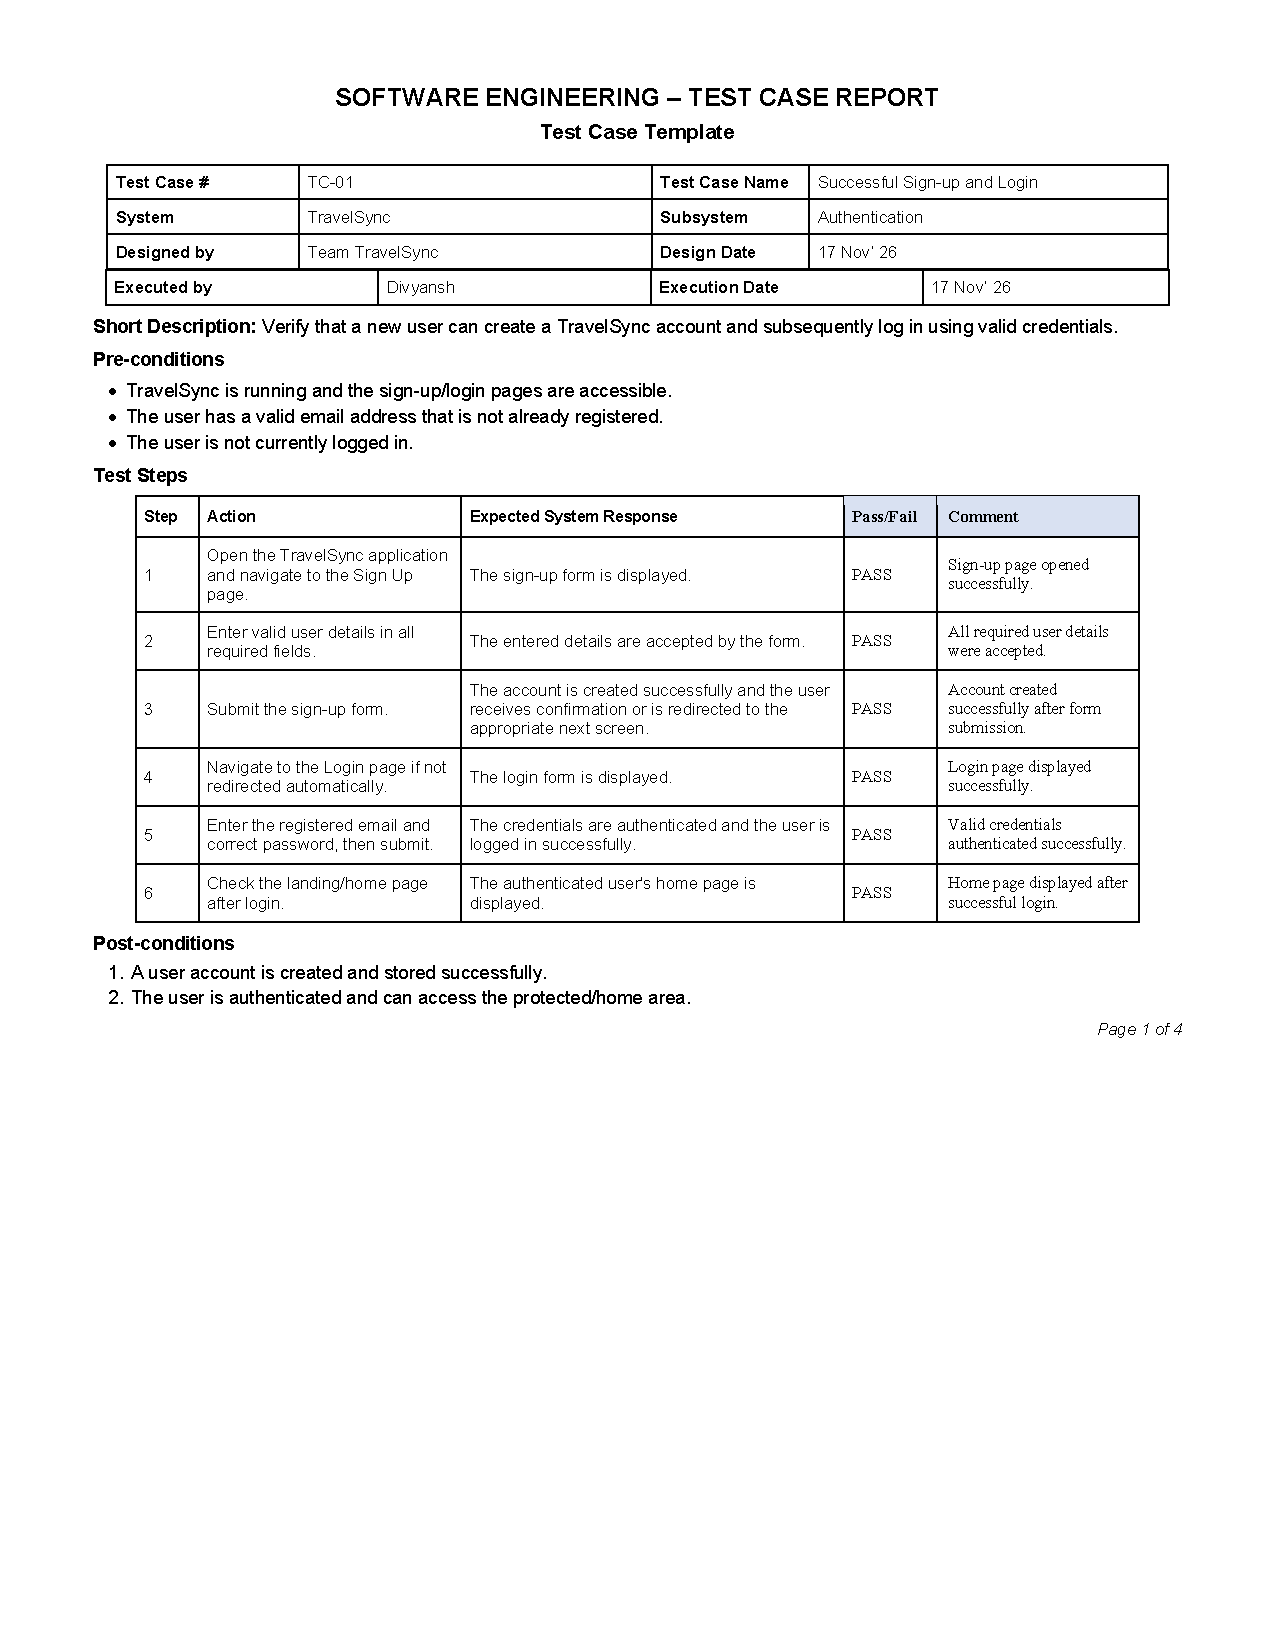
\includegraphics[page=1,width=\textwidth,trim=40 305 41 54,clip]{test_cases.pdf}
  \caption{Test case TC-01: Successful Sign-up and Login}
  \label{tab:tc01}
\end{table}

% Course test-case template, page 2 of figures/test_cases.pdf
\begin{table}[htbp]
  \centering
  \includegraphics[page=2,width=\textwidth,trim=40 288 41 54,clip]{test_cases.pdf}
  \caption{Test case TC-02: Destination Prediction}
  \label{tab:tc02}
\end{table}

% Course test-case template, page 3 of figures/test_cases.pdf
\begin{table}[htbp]
  \centering
  \includegraphics[page=3,width=\textwidth,trim=40 283 41 54,clip]{test_cases.pdf}
  \caption{Test case TC-03: Packing and Health Recommendations}
  \label{tab:tc03}
\end{table}

% Course test-case template, page 4 of figures/test_cases.pdf
\begin{table}[htbp]
  \centering
  \includegraphics[page=4,width=\textwidth,trim=40 319 41 54,clip]{test_cases.pdf}
  \caption{Test case TC-04: Top 5 Places and Stay Recommendations}
  \label{tab:tc04}
\end{table}

\section{Performance Metrics}
\label{sec:performance}

Response times were measured on a running instance of TravelSync on an
Apple MacBook Air (13-inch, 2025) with an Apple M4 processor (10 CPU cores)
and 16\,GB of memory, running macOS~26.5 and Python~3.14. The backend ran as a single Uvicorn worker process
with the in-memory MongoDB-compatible database employed by the test
suite and four registered users with trips, a group, chat messages,
suggestions, votes and bookings. Each endpoint was called 10 times to warm
up and then 200 times sequentially; login was measured over 20 calls.
Because the database ran in the same process, these figures measure the
application's own processing and exclude network latency to a MongoDB
server. Table~\ref{tab:performance} reports the results.

\begin{table}[htbp]
\centering
\begin{tabular}{|l|r|r|}
  \hline
  \textbf{Endpoint} & \textbf{Median} & \textbf{95th percentile} \\
  \hline
  \texttt{GET /api/health} & $0.5$\,ms & $0.6$\,ms \\
  \hline
  \texttt{GET /api/trips} & $0.7$\,ms & $0.7$\,ms \\
  \hline
  \texttt{GET /api/trips/\{id\}/packing-list} & $0.7$\,ms & $0.8$\,ms \\
  \hline
  \texttt{GET /api/groups/\{id\}/messages} & $0.8$\,ms & $0.9$\,ms \\
  \hline
  \texttt{GET /api/bookings} & $0.8$\,ms & $1.9$\,ms \\
  \hline
  \texttt{GET /api/places/\{destination\}} & $1.0$\,ms & $1.2$\,ms \\
  \hline
  \texttt{GET /api/destinations/search} & $1.0$\,ms & $1.1$\,ms \\
  \hline
  \texttt{POST /api/chat} & $1.4$\,ms & $1.4$\,ms \\
  \hline
  \texttt{POST /api/recommend} & $2.2$\,ms & $2.6$\,ms \\
  \hline
  \texttt{GET /api/travel-health/\{destination\}} & $5.2$\,ms & $5.4$\,ms \\
  \hline
  \texttt{POST /api/auth/login} & $167.7$\,ms & $168.4$\,ms \\
  \hline
\end{tabular}
\caption{API response times}
\label{tab:performance}
\end{table}

Throughput was measured on the same instance with 16 concurrent clients,
each sending requests back to back for 10 seconds per endpoint. The load
generator ran on the same laptop as the server, so the figures are a
conservative estimate for a single worker process. No request failed during
any run. Table~\ref{tab:throughput} reports the results.

\begin{table}[htbp]
\centering
\begin{tabular}{|l|r|r|}
  \hline
  \textbf{Endpoint} & \textbf{Throughput} & \textbf{Errors} \\
  \hline
  \texttt{POST /api/chat} & $830.8$\,req/s & $0$ \\
  \hline
  \texttt{GET /api/trips} & $740.8$\,req/s & $0$ \\
  \hline
  \texttt{GET /api/places/\{destination\}} & $730.4$\,req/s & $0$ \\
  \hline
  \texttt{GET /api/groups/\{id\}/messages} & $728.3$\,req/s & $0$ \\
  \hline
  \texttt{POST /api/recommend} & $491.2$\,req/s & $0$ \\
  \hline
  \texttt{GET /api/travel-health/\{destination\}} & $186.5$\,req/s & $0$ \\
  \hline
\end{tabular}
\caption{API throughput with 16 concurrent clients}
\label{tab:throughput}
\end{table}

The accuracy of the recommendation engine was measured as
\emph{precision at five} (Precision@5), the share of the top five
recommendations that are relevant to the request. For each of the twelve
interests, a request selecting only that interest at the highest importance
was issued once for each of the four traveller types (48 requests in total),
and a recommended destination was counted as relevant when its dataset score
for the selected interest was at least 0.5 on the 0--1 scale. Constraint
adherence and engine speed were measured separately over 300 randomly
generated requests from Ludhiana with random interests, importances,
traveller types, durations of 2 to 10 days, budgets from INR~10{,}000 to
INR~80{,}000 and maximum distances from 300 to 2{,}000\,km.
Table~\ref{tab:engine} summarises all evaluation metrics.

\begin{table}[htbp]
\centering
\begin{tabular}{|l|r|}
  \hline
  \textbf{Metric} & \textbf{Measured} \\
  \hline
  Precision@5 (relevance threshold 0.5) & $97.5\%$ (234 of 240) \\
  \hline
  Precision@5 (stricter threshold 0.7) & $86.3\%$ (207 of 240) \\
  \hline
  Top-ranked result relevant (threshold 0.5) & $100\%$ (48 of 48) \\
  \hline
  Relevant share of all destinations (random baseline) & $57.0\%$ \\
  \hline
  Recommendations within the stated maximum distance & $97.8\%$
    (1{,}508 of 1{,}542) \\
  \hline
  Recommendations within the 10\% distance tolerance & $100\%$ \\
  \hline
  Recommendations above 125\% of the stated budget & $0$ \\
  \hline
  Engine time per request, median / 95th percentile & $1.4$\,ms /
    $1.6$\,ms \\
  \hline
  Peak API throughput (one worker) & $830.8$\,req/s \\
  \hline
  Frontend JavaScript bundle (raw / gzip) & $448.0$\,kB / $129.8$\,kB \\
  \hline
  Automated tests passing (backend / frontend) & $196/196$ \,/\,
    $107/107$ \\
  \hline
\end{tabular}
\caption{Summary of evaluation metrics}
\label{tab:engine}
\end{table}

Precision@5 is reported instead of classification accuracy because a
recommender has no single correct answer for a request: a destination can
only be judged relevant or not relevant to it. All six non-relevant results
had a suitability score of at least 0.85 for the requested traveller type,
which shows the traveller-type weighting discussed in
Section~\ref{sec:analysis}.


\section{Analysis}
\label{sec:analysis}

\textbf{Did the project meet its objectives?} All four objectives were met.
Objective~1 is delivered by known-destination selection and the
recommendation engine, which returns explained rankings in a few
milliseconds and stays within the stated distance and budget limits.
Objective~2 is delivered by the trip workspace, which brings together the
top places, packing list, stays, health information and map for each trip.
Objective~3 is delivered by groups with invite codes, live chat, structured
suggestions, single-vote voting and an owner-confirmed decision.
Objective~4 is delivered by bookings with private files, upcoming and
previous trip views, notifications, the assistant, and the security model
verified by the authorisation tests.

\textbf{Where did the project exceed expectations?} The final system goes
beyond the mid-semester plan in several respects: live WebSocket delivery
with read receipts, unread counts and live voting updates; private file
attachments for bookings; a trip map with driving distances; trip editing;
password recovery; and a security design that includes token revocation,
login throttling, cross-site request checks and a production configuration
guard. A total of 303 automated tests pass, the recommender reaches a
Precision@5 of 97.5\%, and every interactive endpoint except deliberately
slow password hashing responds in under 6\,ms and sustains at least
186 requests per second on a single worker in the measured setting.

\textbf{What challenges were encountered?} The main challenges were:
\begin{itemize}
  \item \textbf{Free external-service quotas:} accommodation and routing
    providers limit daily requests, and live hotel prices are not available
    from open data.
  \item \textbf{Real-time consistency:} chat, votes and decisions must stay
    consistent when several members act at once or when a socket
    disconnects.
  \item \textbf{Concurrency and data integrity:} simultaneous requests could
    create duplicate packing lists, duplicate votes or an over-full group.
  \item \textbf{Ranking balance:} with a single interest selected, the fixed
    traveller-type weight can dominate the ranking; for Culture with the
    Solo type, the top five averaged a Culture score of 0.51, below the
    dataset mean of 0.62.
\end{itemize}

\textbf{How were they resolved?} Provider results are cached in MongoDB with
TTL indexes, live lookups are rate-limited per user, coordinates are rounded
before caching, and every provider failure degrades to a clear message or a
local fallback; prices are presented honestly as labelled estimates. Live
updates are sent only after the database write succeeds, and polling remains
as a fallback that catches up after a reconnection. Unique indexes and
atomic conditional updates enforce one packing list per trip, one vote per
member and the twenty-member group limit. The traveller-type weighting is
identified as a tuning target in Section~\ref{sec:future-work}.

The remaining limitations of the current version are that the chat hub keeps
socket connections in one process, so horizontal scaling would require a
shared message broker; that health alerts are curated by hand rather than
received from a live feed; that the recommendation weights were set by
design judgement rather than learned from user feedback; and that the
system has not yet been evaluated in a formal user study.
